\section{Implementation}
This section will outline the employed software and hardware resources of the system, explain the data preprocessing, and describe the model architecture of our neural networks in detail.

\subsection{Software}
\label{sec:software}


	The language identification system is implemented in Python. We used the open source deep learning framework Keras\cite{chollet2015keras} with the TensorFlow\cite{abadi2016tensorflow} backend for training our neural networks. Keras provides us with a set of higher level machine learning primitives such as convolutional layers and optimizing algorithms without abstracting too much away. Internally it builds on Google's open source numerical operation library TensorFlow which is optimized to quickly compute large multidimensional data on GPUs.
		
	 
	From a high level perspective, our system was designed in three parts. 
	
	\begin{description}
		\item[The preprocessor] Its job is to download, extract, and convert the data. The preprocessor clips the audio tracks for raw video footage and converts them into WAV files before ultimately converting the data into PNG images for the training. Details can be found in section \ref{sec:data_processing}.
		\item[The trainer]
		\item[The evaluator] 
	\end{description}
	

\subsection{Data Preprocessing}
\label{sec:data_processing}
All audio files have to be preprocessed before feeding them to the neural network. As a first step all files are encoded as uncompressed, lossless Waveform Audio File Format\footnote{\url{http://www.microsoft.com/whdc/device/audio/multichaud.mspx}, accessed 23.02.2017}, WAVE, commonly know by its file extension *.wav. This conversion has two advantages: A lossless data codec allows for future audio manipulations with any quality loss and makes the data easily readable by third party programs and library such as SciPy\footnote{\url{https://www.scipy.org/}, accessed 23.02.2017}. 

	Since our CNN does not operate on raw waveform audio signals we transfer it into the image domain. As introduced in section \ref{sec:audio_representations} we used a spectrogram representation of the audio file for model training. The spectrograms were generated using the open source command line tool SoX\footnote{\url{http://sox.sourceforge.net/}, accessed 23.02.2017}. Spectrograms are generated using a Hann window and 129 frequency bins along the frequency-axis (y-axis). The time-axis (x-axis) is rendered at 25 pixel per second. Each audio sequence is clipped into non-overlapping ten second segments. The  final segment is discarded to avoid segments shorter than the required ten seconds. We decided against filtering silent section within the audio segment to keep the natural pauses between words and not disturb the regular speech rhythm. Frequency intensities are mapped to a gray scale. The resulting greyscale images are saved as lossless PNG files and are 500 pixel in width and 129 pixel in height. Appendix \ref{sec:appendix_a} includes the complete listing \ref{lst:spectrograms} for generating spectrogram images with SoX.
	
	As can be seen in figure \ref{fig:spectrogram} the spectrograms feature very apparent bright ripple-like pattern. Each of these represents a strong activation of a certain frequency over time. Several frequency activations can be active at once constituting a particular phoneme or sound. A sequence of these phonemes forms words and is only interrupted by short speech pauses. It is our aim to learn the characteristic and unique composition of these frequency activation for every language in our classifier. 

	
	\begin{figure}[h]
  		\centering
    	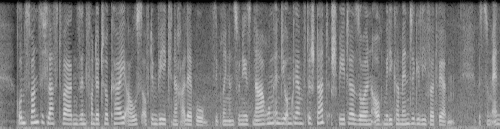
\includegraphics[width=\textwidth,keepaspectratio]{img/spectrogram.png}
    	\caption{A spectrogram generated from a ten second German audio clip  using SoX. Notice the bright ripple-like patterns. These frequency activations serve as the main features for the classifier.}
    	\label{fig:spectrogram}
	\end{figure}
	
    \begin{itemize}
        \item Spectrogram Generation
        \item Data Segmentation
        \item (Augmentation)
        \item train / test split
		\item number of training samples
    \end{itemize}

\subsection{CNN Architecture}


    \begin{itemize}
        \item Layer Table
        \item Transfer Learning / Fine-tuning
        \item Variations
    \end{itemize}
    
    \begin{table}[h]
  \centering
  \begin{tabularx}{\textwidth}{Xllll}
  \toprule
  Layer Type                       & input maps  & output maps & kernel & stride  \\ \midrule
  \mbox{Convolution with} \mbox{Batch Normalization}  & 1           & 16     & 7x7    & 1       \\ 
  Max Pooling                           & 16          & 16     & 2x2    & 2       \\ 
  Convolution with Batch Normalization  & 16          & 32     & 5x5    & 1       \\ 
  Max Pooling                           & 32          & 32     & 2x2    & 2       \\ 
  Convolution with Batch Normalization  & 32          & 64     & 3x3    & 1       \\ 
  Max Pooling                           & 64          & 64     & 2x2    & 2       \\ 
  Convolution with Batch Normalization  & 64          & 128    & 3x3    & 1       \\ 
  Max Pooling                           & 128         & 128    & 2x2    & 2       \\ 
  Convolution with Batch Normalization  & 128         & 256    & 3x3    & 1       \\ 
  Max Pooling                           & 256         & 256    & 2x2    & 2       \\ 
  Dropout                               &             &        &        &         \\ 
  Fully Connected                       & ???         & 1024   &        &         \\ 
  Fully Connected                       & 1024        & 4      &        &        \\ 
  \bottomrule
  \end{tabularx}
  \caption{The layer architecture for the convolutional neural network CNN\_A.}
  \label{tab:layers_CNN_A}
  \end{table}
    
    

\subsection{CRNN Architecture}

    \begin{itemize}
        \item Layer Table
        \item Architecture Image
        \item Conv Features to time steps
        \item Transfer Learning / Fine-tuning
        \item 
    \end{itemize}
